\chapter{化学势与混合物}\label{ch:b2:chemical-potential}

冬天，撒盐车在结冰的路面上撒盐，冰在 \qty{-10}{\celsius} 时即融化；
汽车发动机的冷却液是水与三分之一的 1,2-乙二醇的混合物，
在夜间霜冻中不结冰，在发热的引擎盖下也不沸腾。
溶解的物质会降低溶剂的凝固点、提高其沸点，
而对稀溶液而言，这一变化量
只取决于溶解粒子的数目，而与粒子是什么无关。
解释这一现象的工具是\omterm{def:b2:chemical-potential:chemical-potential}{化学势}，
即\omterm{def:b2:reaction-free-energy:gibbs-energy}{吉布斯自由能}对某一组分物质的量的偏导数。
它说明各物种“想要去哪里”，无论是在相与相之间，还是通过反应；
它还把本科一年级分册中当作配方使用的活度，
转化为导出量。

\begin{recall}
\Cref{ch:b2:reaction-free-energy}中的\omterm{def:b2:reaction-free-energy:gibbs-energy}{吉布斯自由能} $G = H - TS$，$\dd G =
V\dd p - S\dd T + \Delta_r G\,\dd\xi$，演变判据 $\Delta_r G\,
\dd\xi \leq 0$。本科一年级分册将气体的活度写作
$p_i/p^\circ$，溶质写作 $c_i/c^\circ$，纯固体或
溶剂取 1，并指出在浓的离子溶液中，活度
与浓度有偏离，“这一修正将在本科二年级分册中处理”。由物理学可知
：理想气体定律，以及对纯物质
有 $(\partial G/\partial p)_T = V$。
\end{recall}

\begin{omfigure}

\includegraphics[width=0.58\linewidth]{images/book3/ai/b2-03-salt-spreader.jpg}

{\small 撒盐车在积雪的路面上撒盐。盐溶解于冰面上的薄水膜中，
溶液的凝固温度低于纯水，
于是冰融化。}
\end{omfigure}

\section{偏摩尔量}

将 \qty{50}{mL} 水与 \qty{50}{mL} 乙醇混合，混合物的体积
小于 \qty{100}{mL}。在混合物中，广延量
并不等于各纯物质贡献之和；每一组分的贡献
取决于它所处的环境。

\begin{definition}[偏摩尔量]\label{def:b2:chemical-potential:partial-molar}
设 $X(T, p, n_1, \dots, n_k)$ 为某一相的广延状态函数，
该相含有物质的量 $n_1, \dots, n_k$。
组分 $i$ 的\emph{偏摩尔量}\index{偏摩尔量}定义为
\[
  \bar X_i = \left(\frac{\partial X}{\partial n_i}\right)_{T, p, n_{j \ne i}} ,
\]
即 $X$ 相对于向大量混合物中每加入 1 摩尔 $i$ 的变化，
在温度 $T$、压强 $p$ 及其他物质的量固定的条件下。对于 $X = V$，它称为\emph{偏摩尔体积}\index{偏摩尔体积}
记作 $\bar V_i$。
\end{definition}

\begin{theorem}[欧拉恒等式]\label{thm:b2:chemical-potential:euler}
在温度 $T$ 与压强 $p$ 固定时，$X = \sum_i n_i\bar X_i$。
\end{theorem}

\begin{proof}
$X$ 为广延量：每个物质的量乘以 $\lambda$，$X$ 也乘以
$\lambda$，即 $X(T, p, \lambda n_1, \dots, \lambda n_k) = \lambda X(T, p, n_1,
\dots, n_k)$。对 $\lambda$ 在 $\lambda = 1$ 处求导，并
用链式法则，得 $\sum_i n_i\,\partial X/\partial n_i = X$。
\end{proof}

\begin{proposition}[吉布斯–杜安关系]\label{prop:b2:chemical-potential:gibbs-duhem}
在温度 $T$ 与压强 $p$ 固定时，$\sum_i n_i\,\dd\bar X_i = 0$；对二元混合物，
$x_1\dd\bar X_1 + x_2\dd\bar X_2 = 0$。各组分的\omterm{def:b2:chemical-potential:partial-molar}{偏摩尔量}
不能彼此独立地变化。
\end{proposition}

\begin{proof}
在 $T$、$p$ 固定时，由定义 $\dd X = \sum_i\bar X_i\dd n_i$；
对欧拉恒等式求微分，得 $\dd X = \sum_i\bar X_i\dd n_i + \sum_i
n_i\dd\bar X_i$。两式相减即得。
\end{proof}

\begin{omfigure}
\begin{tikzpicture}
\begin{axis}[
  width=0.62\linewidth, height=5.4cm, xmin=0, xmax=1, ymin=8, ymax=62,
  axis x line=bottom, axis y line=left, xlabel={摩尔分数 $x_2$},
  ylabel={摩尔体积 $V_m$（模型）}, xtick={0,0.2,0.4,0.6,0.8,1}, ytick=\empty,
  tick label style={font=\small}, label style={font=\small}, ylabel shift=10pt, clip=false]
\addplot[omDef, very thick, domain=0:1, samples=60] {18*(1-x) + 58*x - 25*x*(1-x)};
\addplot[black!40, dashed, domain=0:1] {18*(1-x) + 58*x};
\addplot[omThm, thick, domain=0:1] {14 + 35*x};
\fill[omThm] (axis cs:0.4,28) circle (1.6pt);
\node[omThm, anchor=east, font=\small] at (axis cs:-0.01,14) {$\bar V_1$};
\node[omThm, anchor=west, font=\small] at (axis cs:1,49) {$\bar V_2$};
\node[font=\scriptsize, anchor=south east, black!60] at (axis cs:0.62,44) {纯组分体积相加};
\node[font=\small, anchor=north west] at (axis cs:0.41,27) {$x_2 = 0.4$};
\end{axis}
\end{tikzpicture}

{\small 切线作图。二元模型混合物的摩尔体积（蓝色）
位于连接两纯物质体积的直线下方，混合时体积收缩。
某组成处的切线与两端相交，交点给出该组成下的
\omterm{def:b2:chemical-potential:partial-molar}{偏摩尔体积} $\bar V_1$ 与 $\bar V_2$。}
\end{omfigure}

\begin{method}[由曲线求偏摩尔量]\label{met:b2:chemical-potential:tangent}
以摩尔量 $X_m = X/(n_1 + n_2)$ 对 $x_2$ 作图。在
所关心的组成处作切线：切线与轴 $x_2 = 0$ 相交于
$\bar X_1$，与轴 $x_2 = 1$ 相交于 $\bar X_2$。（证明：$X_m = x_1\bar X_1 +
x_2\bar X_2$，由吉布斯–杜安关系，$\dd X_m/\dd x_2 = \bar X_2 - \bar X_1$。）
\end{method}

\section{化学势}

\begin{definition}[化学势]\label{def:b2:chemical-potential:chemical-potential}
组分 $i$ 在某相中的\emph{化学势}\index{化学势}
为其偏摩尔\omterm{def:b2:reaction-free-energy:gibbs-energy}{吉布斯自由能}，即
\[
  \mu_i = \left(\frac{\partial G}{\partial n_i}\right)_{T, p, n_{j\ne i}} ,
\]
单位为 \unit{J/mol}。当 $i$ 处于标准状态时的值，称为其
\emph{标准化学势}\index{标准化学势}
$\mu_i^\circ(T)$，等于 $i$ 的标准摩尔\omterm{def:b2:reaction-free-energy:gibbs-energy}{吉布斯自由能}。
\end{definition}

对于物质的量可以改变的相（通过反应，或与
另一相交换物质），有
\[
  \dd G = V\dd p - S\dd T + \sum_i\mu_i\,\dd n_i ,\qquad G = \sum_i n_i\mu_i ,
\]
其中第二式由欧拉恒等式得到。对于单一反应，$\dd n_i =
\nu_i\dd\xi$，与\cref{prop:b2:reaction-free-energy:dG}比较，得
\[
  \Delta_r G = \sum_i\nu_i\mu_i .
\]
\omterm{def:b2:reaction-free-energy:reaction-gibbs}{反应吉布斯自由能}是生成物与
反应物\omterm{def:b2:chemical-potential:chemical-potential}{化学势}之差。

\begin{theorem}[相间平衡]\label{thm:b2:chemical-potential:phase-equilibrium}
在闭合系统中，某组分同时存在于两相 $\alpha$ 与 $\beta$ 中，
两相的温度 $T$ 与压强 $p$ 均匀时，该组分在两相间处于平衡的充要条件是
$\mu_i^\alpha = \mu_i^\beta$。否则，它会自发地从\omterm{def:b2:chemical-potential:chemical-potential}{化学势}较高的相
转移到\omterm{def:b2:chemical-potential:chemical-potential}{化学势}较低的相。
\end{theorem}

\begin{proof}
转移过程 $i^\alpha \to i^\beta$ 是一个“反应”，其中 $\nu^\alpha = -1$，
$\nu^\beta = +1$，故 $\Delta_r G = \mu_i^\beta - \mu_i^\alpha$。由
演化判据，过程正向进行（$\dd\xi > 0$）的条件是 $\mu_i^\beta <
\mu_i^\alpha$，逆向进行的条件是 $\mu_i^\beta > \mu_i^\alpha$，
二者相等时处于平衡。
\end{proof}

\omterm{def:b2:chemical-potential:chemical-potential}{化学势}之于物质，犹如温度之于热量：
热量由高温流向低温，物种则由 $\mu$ 高处流向低处。

\section{理想体系与活度}

\begin{proposition}[理想气体的化学势]\label{prop:b2:chemical-potential:mu-gas}
在理想气体混合物中，分压为 $p_i$ 的气体具有
\[
  \mu_i = \mu_i^\circ(T) + RT\ln\frac{p_i}{p^\circ} .
\]
\end{proposition}

\begin{proof}
对于一摩尔纯理想气体，有 $(\partial\mu/\partial p)_T = V_m =
RT/p$；从 $p^\circ$ 积分到 $p$，得 $\mu = \mu^\circ + RT\ln(p/p^\circ)$。
在理想气体混合物中，每种气体的行为如同单独占据该体积，且处于
其分压：将 $p$ 替换为 $p_i$ 即可。
\end{proof}

\begin{definition}[理想混合物，理想稀溶液]\label{def:b2:chemical-potential:ideal-mixture}
若液态（或固态）混合物对每一组分及每一组成均满足下式，
则称其为\emph{理想混合物}\index{理想混合物}：
$\mu_i = \mu_i^*(T, p) + RT\ln x_i$，其中 $\mu_i^*$ 为纯液体 $i$ 的\omterm{def:b2:chemical-potential:chemical-potential}{化学势}。
溶液称为\emph{理想稀溶液}\index{理想稀溶液}，若其溶剂服从此定律，且
每种溶质满足
$\mu_j = \mu_j^\circ(T) + RT\ln(c_j/c^\circ)$，其中标准状态为
$c^\circ = \qty{1}{mol/L}$ 的假想溶液，
其行为如同无限稀释。
\end{definition}

大小和形状相近、相互作用与伙伴无关的分子，
（例如苯与甲苯、同一分子的两种同位素形式）近似形成\omterm{def:b2:chemical-potential:ideal-mixture}{理想混合物}；
稀溶液表现出理想行为，因为每个溶质
粒子周围只有溶剂分子。

\begin{theorem}[拉乌尔定律]\label{thm:b2:chemical-potential:raoult}
在理想液体混合物上方，若蒸气为理想气体，则每一组分的分压
与其在液相中的摩尔分数成正比：$p_i = x_i\,p_i^*$，
其中 $p_i^*$ 为同一温度下纯液体的蒸气压
（\emph{拉乌尔定律}\index{拉乌尔定律}）。
\end{theorem}

\begin{proof}
平衡时 $\mu_i(\text{液体}) = \mu_i(\text{蒸气})$：$\mu_i^* +
RT\ln x_i = \mu_i^\circ + RT\ln(p_i/p^\circ)$。对于纯液体（$x_i = 1$，
$p_i = p_i^*$）：$\mu_i^* = \mu_i^\circ + RT\ln(p_i^*/p^\circ)$。两式相减，
得 $RT\ln x_i = RT\ln(p_i/p_i^*)$。（忽略 $\mu_i^*$ 对
压强的微弱依赖。）
\end{proof}

\begin{proposition}[亨利定律]\label{prop:b2:chemical-potential:henry}
对于与其蒸气处于平衡的稀溶质 $j$，有 $p_j = k_{H,j}\,x_j$
（或 $c_j = H_j\,p_j$）：稀溶质的分压
与其在溶液中的物质的量成正比（\emph{亨利定律}\index{亨利定律}）。
其\emph{亨利常数}\index{亨利常数}
$k_{H,j}$ 取决于溶质、溶剂与温度，
且不等于纯溶质的蒸气压。
\end{proposition}

\begin{proof}
令 $\mu_j^\circ(\text{溶液}) + RT\ln(c_j/c^\circ)$ 与
$\mu_j^\circ(\text{气体}) + RT\ln(p_j/p^\circ)$ 相等，$c_j/p_j$ 仅
是 $T$ 的函数。该常数包含 $j$ 与溶剂的相互作用，而非
它与自身的相互作用。
\end{proof}

\begin{omfigure}
\begin{tikzpicture}
\begin{axis}[name=a,
  width=0.48\linewidth, height=5.6cm, xmin=0, xmax=1, ymin=0, ymax=1.5,
  axis x line=bottom, axis y line=left, xlabel={$x_1$}, ylabel={$p/p_1^*$},
  xtick={0,0.5,1}, ytick={0,0.5,1,1.5},
  tick label style={font=\small}, label style={font=\small}, title={\small 理想}]
\addplot[omDef, thick] table[x=x1, y=p1] {figdata/out/bachelor-2-raoult-henry-ideal.dat};
\addplot[omThm, thick] table[x=x1, y=p2] {figdata/out/bachelor-2-raoult-henry-ideal.dat};
\addplot[black, very thick] table[x=x1, y=p] {figdata/out/bachelor-2-raoult-henry-ideal.dat};
\node[omDef, font=\scriptsize, anchor=west] at (axis cs:0.55,0.42) {$p_1$};
\node[omThm, font=\scriptsize, anchor=west] at (axis cs:0.1,0.42) {$p_2$};
\node[font=\scriptsize, anchor=south] at (axis cs:0.5,0.8) {$p$};
\end{axis}
\begin{axis}[at={(a.east)}, anchor=west, xshift=1.2cm,
  width=0.48\linewidth, height=5.6cm, xmin=0, xmax=1, ymin=0, ymax=1.5,
  axis x line=bottom, axis y line=left, xlabel={$x_1$},
  xtick={0,0.5,1}, ytick={0,0.5,1,1.5},
  tick label style={font=\small}, label style={font=\small}, title={\small 正偏差}]
\addplot[omDef, thick] table[x=x1, y=p1] {figdata/out/bachelor-2-raoult-henry-margules.dat};
\addplot[omThm, thick] table[x=x1, y=p2] {figdata/out/bachelor-2-raoult-henry-margules.dat};
\addplot[black, very thick] table[x=x1, y=p] {figdata/out/bachelor-2-raoult-henry-margules.dat};
\addplot[omDef, densely dashed, domain=0.6:1] {x};
\addplot[omDef, dotted, thick, domain=0:0.42] {3.004166*x};
\node[omDef, font=\scriptsize, anchor=west] at (axis cs:0.62,0.5) {拉乌尔};
\node[omDef, font=\scriptsize, anchor=east] at (axis cs:0.27,1.18) {亨利};
\node[omDef, font=\scriptsize, anchor=north west] at (axis cs:0.8,0.78) {$p_1$};
\node[omThm, font=\scriptsize, anchor=north] at (axis cs:0.55,0.24) {$p_2$};
\node[font=\scriptsize, anchor=south] at (axis cs:0.5,1.23) {$p$};
\end{axis}
\end{tikzpicture}

{\small 固定温度下二元液体上方的蒸气压，以
$p_1^*$ 为单位（模型混合物）。左图为\omterm{def:b2:chemical-potential:ideal-mixture}{理想混合物}：直线（拉乌尔）。
右图为异种分子之间的相互吸引弱于同种分子的混合物，
压强位于理想直线之上。在 $x_1 = 1$ 附近，组分 1
遵循拉乌尔直线（虚线）；在 $x_1 = 0$ 附近，它遵循
斜率不同的亨利直线（点线）。}
% (computed in figdata/bachelor-2/raoult-henry.py; Margules parameter 1.1, model)
\end{omfigure}

\begin{example}[二氧化碳在汽水中]\label{ex:b2:chemical-potential:soda}
在 \qty{25}{\celsius} 下，二氧化碳在水中的\omterm{prop:b2:chemical-potential:henry}{亨利常数}为 $H =
\qty{3.4e-4}{mol/(m^3.Pa)}$，即 \qty{0.034}{mol/(L.bar)}。
密封于 \qty{4}{bar} 的 \ce{CO2} 之下的瓶中，溶解气体的量为 $0.034 \times 4 =
\qty{0.14}{mol/L}$ 的溶解气体，约合 \qty{6}{g/L}。开启后，瓶中上方的
气体即为空气，其中 $p_{\ce{CO2}} \approx \qty{4e-4}{bar}$，饮料的
过饱和程度约为一万倍，直至气泡逸尽而变平淡。
% ledger: henry:CO2, air:CO2
\end{example}

\begin{proposition}[由化学势求活度]\label{prop:b2:chemical-potential:activity}
在迄今所遇到的各种情形中，$\mu_i = \mu_i^\circ(T) + RT\ln a_i$，其中 $a_i$
为本科一年级分册中的活度：对理想气体为 $p_i/p^\circ$，
对\omterm{def:b2:chemical-potential:ideal-mixture}{理想稀溶液}中的溶质为 $c_i/c^\circ$，
对溶剂为 $x_i$（接近 1），对单独存在于其相中的纯固体或纯液体为 1。
\end{proposition}

\begin{proof}
对于气体和稀溶液中的溶质，此即
\cref{prop:b2:chemical-potential:mu-gas} 的内容，以及
\omterm{def:b2:chemical-potential:ideal-mixture}{理想稀溶液}的定义。对于\omterm{def:b2:chemical-potential:ideal-mixture}{理想混合物}的组分，取其标准
状态为纯液体：$a_i = x_i$，对溶剂而言接近 1。纯固体
或纯液体以自身为标准状态，
忽略其对压强的微弱依赖：$\mu = \mu^\circ$，$a = 1$。
\end{proof}

\begin{proposition}[反应吉布斯自由能与反应商]\label{prop:b2:chemical-potential:delta-g-q}
对于反应 $0 = \sum_i\nu_i\mathrm A_i$，
\[
  \Delta_r G = \Delta_r G^\circ(T) + RT\ln Q, \qquad Q = \prod_i a_i^{\nu_i} .
\]
\end{proposition}

\begin{proof}
$\Delta_r G = \sum_i\nu_i\mu_i = \sum_i\nu_i\mu_i^\circ + RT\sum_i\nu_i\ln a_i =
\Delta_r G^\circ + RT\ln\prod_i a_i^{\nu_i}$.
\end{proof}

这是 \cref{ch:b2:reaction-free-energy} 中的\omterm{def:b2:reaction-free-energy:gibbs-energy}{吉布斯自由能}与
本科一年级分册中的反应商之间的桥梁。下一章即跨越此桥。

\begin{method}[选取活度的参考态]\label{met:b2:chemical-potential:activity-reference}
\begin{enumerate}
  \item 气体：$p^\circ$ 下的纯理想气体；$a = p_i/p^\circ$。
  \item 溶剂，或量相当的混合物中的组分：
        纯液体；$a = \gamma_i x_i$（拉乌尔参考态，$\gamma_i \to 1$
        当 $x_i \to 1$ 时）。
  \item 溶质：$c^\circ$ 下的理想溶液；$a = \gamma_j c_j/c^\circ$
        （亨利参考态，$\gamma_j \to 1$，当无限稀释时）。
  \item 纯固体，单独存在于其相中的纯液体：$a = 1$。
\end{enumerate}
\end{method}

\begin{history}[弗朗索瓦-玛丽·拉乌尔]
\begin{minipage}[t]{0.2\linewidth}\vspace{0pt}
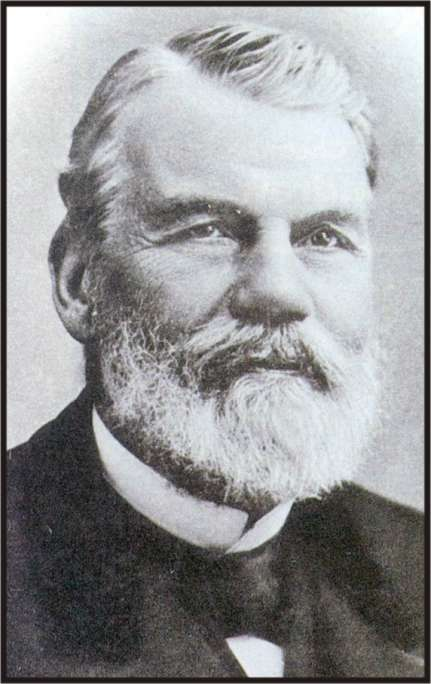
\includegraphics[width=\linewidth]{images/book3/raoult.jpg}
\end{minipage}\hfill
\begin{minipage}[t]{0.76\linewidth}\vspace{0pt}
弗朗索瓦-玛丽·拉乌尔（1830--1901），格勒诺布尔大学化学教授，
于 1880 年代先后测量了数百种溶液的凝固点和蒸气压，
发现对于稀溶液而言，凝固点的降低
仅取决于溶解分子的数目，而与其本性无关。他的
测量成为一种称量分子的方法，并支持了年轻的
溶液中离子理论。（照片：公有领域，维基共享资源。）
\end{minipage}
\end{history}

\section{真实混合物}

\begin{definition}[活度系数]\label{def:b2:chemical-potential:activity-coefficient}
在真实混合物中，\omterm{def:b2:chemical-potential:chemical-potential}{化学势}写为 $\mu_i = \mu_i^\circ +
RT\ln a_i$，其中 $a_i = \gamma_i x_i$（拉乌尔参考态）或 $a_i = \gamma_i
c_i/c^\circ$（亨利参考态）。因子 $\gamma_i$ 称为
\emph{活度系数}\index{活度系数}：它度量
偏离理想定律的程度，并在参考定律成立的极限下趋于 1。
\end{definition}

系数大于 1 意味着，分子在混合物中受邻近分子的稳定作用
比在参考态中弱（正偏差，如上图所示）；
系数小于 1 则意味着稳定作用更强。由吉布斯–杜安方程，二元混合物两组分的
系数相互关联：在图中所用的单参数模型中，
$\ln\gamma_1 = Ax_2^2$，$\ln\gamma_2 = Ax_1^2$，并且
$x_1\,\dd\ln\gamma_1 + x_2\,\dd\ln\gamma_2 = 0$ 恒成立。

对于离子，由于其相互作用为长程作用，
在较小浓度下即已出现偏离。

\begin{definition}[离子强度]\label{def:b2:chemical-potential:ionic-strength}
溶液的\emph{离子强度}\index{离子强度}为 $I =
\frac12\sum_i z_i^2\,b_i$，其中 $b_i$ 为离子 $i$ 的质量摩尔浓度（每
千克溶剂中的物质的量），$z_i$ 为其电荷数。
\end{definition}

\begin{proposition}[德拜–休克尔极限定律]\label{prop:b2:chemical-potential:debye-huckel}
在极稀的电解质溶液中，盐中离子的平均\omterm{def:b2:chemical-potential:activity-coefficient}{活度系数}
服从 $\log\gamma_\pm = -A\,|z_+z_-|\sqrt{I/b^\circ}$，其中 $A
\approx 0.51$，对于 \qty{25}{\celsius} 下的水，$b^\circ =
\qty{1}{mol/kg}$。
\end{proposition}
\admitted

\begin{remark}[适用范围与来源]\label{rem:b2:chemical-potential:dh-range}
该定律来自一个模型：每个离子被一层带相反电荷的扩散
“大气”所包围，这层大气使其\omterm{def:b2:chemical-potential:chemical-potential}{化学势}降低。该模型超出本课程范围，
但其常数 $A$ 由水的介电常数、密度和温度决定。该定律在约
$I = \qty{0.01}{mol/kg}$ 以下时是准确的。同样的离子大气在电场中
使离子减速，并解释了强电解质的摩尔电导率为何
随 $\Lambda = \Lambda^\circ - K\sqrt c$ 下降（科尔劳施平方根定律），
而不是保持在其极限值：这正是
本科一年级分册中科尔劳施定律所讨论的
极限情形。
% ledger: epsr:H2O, rho:water.298, const:e, const:eps0, const:kB, const:NA (A computed in figdata/bachelor-2/colligative.py)
\end{remark}

\begin{example}[百分之一摩尔浓度的盐]\label{ex:b2:chemical-potential:dh}
对于 $b = \qty{0.010}{mol/kg}$ 的氯化钠，$I = \frac12(0.010 + 0.010)
= \qty{0.010}{mol/kg}$，$\log\gamma_\pm = -0.51 \times 0.10$，于是 $\gamma_\pm
= 0.89$。在每千克百分之一摩尔的浓度下，以浓度代替活度
所造成的误差为 11\,\%；对于 2:2 型盐，如
硫酸镁（同一质量摩尔浓度），$I = 0.040$，$\gamma_\pm = 0.62$。
\end{example}

\section{依数性}

\begin{definition}[依数性]\label{def:b2:chemical-potential:colligative}
稀溶液的\emph{依数性}\index{依数性}是指只取决于单位溶剂中
溶解粒子的物质的量、而与粒子本性无关的性质，
包括蒸气压降低、凝固点降低、沸点升高以及\omterm{def:b2:chemical-potential:osmotic-pressure}{渗透压}。
下文凝固点定律与沸点定律中的常数，
即溶剂的
\emph{凝固点降低常数}\index{凝固点降低常数} $K_f$
与
\emph{沸点升高常数}\index{沸点升高常数} $K_b$。
\end{definition}

\begin{omfigure}
\begin{tikzpicture}[font=\small, >={Stealth}]
  \draw[->] (0,0) -- (8,0) node[right] {$T$};
  \draw[->] (0,0) -- (0,4.4) node[above] {溶剂的 $\mu$};
  % slopes = -S_m: the liquid, more disordered, falls faster than the solid
  \draw[omDef, very thick] (0.4,3.0) -- (7.0,2.01) node[right] {固体};
  \draw[omThm, very thick] (0.4,3.6) -- (7.6,0.72) node[right] {纯液体};
  \draw[omThm, very thick, dashed] (0.4,3.25) -- (7.6,0.37) node[right] {溶液};
  \fill (2.8,2.64) circle (1.5pt);
  \fill (1.4,2.85) circle (1.5pt);
  \draw[densely dotted] (2.8,2.64) -- (2.8,0) node[below] {$T_f^*$};
  \draw[densely dotted] (1.4,2.85) -- (1.4,0) node[below] {$T_f$};
  \draw[<->] (1.4,-0.75) -- (2.8,-0.75) node[midway, below] {$\Delta T_f$};
  \draw[<->, black!70] (5.0,1.76) -- (5.0,1.41);
  \draw[black!50] (5.0,1.58) -- (4.6,0.75) node[below, font=\scriptsize, black] {$RT\ln x_1$};
\end{tikzpicture}

{\small 溶剂的\omterm{def:b2:chemical-potential:chemical-potential}{化学势}随温度的变化（示意图，
固定压强）。稳定相是 $\mu$ 最低者。溶解溶质后，液体的
直线下移 $RT\ln x_1 < 0$，它在更低的温度下与固体的
直线相交：溶液的凝固点低于纯溶剂。}
\end{omfigure}

\begin{theorem}[凝固点降低]\label{thm:b2:chemical-potential:cryoscopy}
若稀溶液中的溶质不进入固体，则溶液开始凝固的温度为
$T_f = T_f^* - \Delta T_f$，其中
\[
  \Delta T_f = K_f\,b, \qquad K_f = \frac{R\,T_f^{*2}\,M_1}{\Delta_{\text{fus}}H_1} ,
\]
$b$ 为溶解粒子的总质量摩尔浓度，$M_1$ 为溶剂的
摩尔质量（单位为 \unit{kg/mol}）。对于有限浓度，理想溶液的精确
关系为 $\ln x_1 = -\frac{\Delta_{\text{fus}}H_1}{R}
\left(\frac{1}{T_f} - \frac{1}{T_f^*}\right)$。
\end{theorem}

\begin{proof}
在凝固点处，纯固态溶剂与溶液中的溶剂处于
平衡：$\mu_1^{\text{s}}(T) = \mu_1^{*\text{l}}(T) + RT\ln x_1$，于是
$\ln x_1 = -\Delta_{\text{fus}}G_1(T)/(RT)$，其中 $\Delta_{\text{fus}}G_1 =
\mu_1^{*\text{l}} - \mu_1^{\text{s}}$，在 $T_f^*$ 处为零。由吉布斯–亥姆霍兹方程，
$\dd(\Delta_{\text{fus}}G_1/T)/\dd T = -\Delta_{\text{fus}}H_1/T^2$；
自 $T_f^*$ 积分至 $T_f$，并取 $\Delta_{\text{fus}}H_1$ 为常数，即得
精确关系。对于稀溶液，$\ln x_1 = \ln(1 - x_2) \approx
-x_2$，且 $\frac1{T_f} - \frac1{T_f^*} \approx -\Delta T_f/T_f^{*2}$，于是
$x_2 = \Delta_{\text{fus}}H_1\Delta T_f/(RT_f^{*2})$；最后 $x_2 \approx
n_2/n_1 = b\,M_1$。
\end{proof}

\begin{proposition}[沸点升高]\label{prop:b2:chemical-potential:ebullioscopy}
含不挥发溶质的稀溶液沸腾于 $T_b^* + \Delta T_b$，
其中 $\Delta T_b = K_b\,b$，$K_b = RT_b^{*2}M_1/\Delta_{\text{vap}}H_1$。
\end{proposition}

\begin{proof}
证明与上面相同，只需以蒸气代替固体：$\mu_1^{*\text{l}} +
RT\ln x_1 = \mu_1^{\text{v}}$；溶剂的直线下移，此时在更高温度下与
蒸气的直线相交。
\end{proof}

\begin{example}[水]\label{ex:b2:chemical-potential:water-constants}
取 $\Delta_{\text{fus}}H = \qty{333.4}{J/g} = \qty{6.007}{kJ/mol}$，
温度为 \qty{273.15}{K}，则 $K_f = 8.314 \times 273.15^2 \times 0.018015/6007 =
\qty{1.86}{K.kg/mol}$。取 $\Delta_{\text{vap}}H = \qty{40.65}{kJ/mol}$，
温度为 \qty{373.12}{K}，则 $K_b = \qty{0.513}{K.kg/mol}$。海水含盐量为 \qty{35}{g}
每千克，按氯化钠计（每个化学式含两个粒子）：
$b = 2 \times 35/58.44/0.965 = \qty{1.24}{mol/kg}$，故稀溶液定律
预测凝固点为 \qty{-2.3}{\celsius}，这是高估：在此浓度下
离子远非理想状态，且海盐并非全部为氯化钠。
% ledger: dfus:H2O, tfus:H2O, dvap:H2O.nbp, tb:H2O.atm, sea:salinity (computed in figdata/bachelor-2/colligative.py)
\end{example}

\begin{definition}[半透膜与渗透压]\label{def:b2:chemical-potential:osmotic-pressure}
\emph{半透膜}\index{半透膜}允许溶剂通过、
而不允许溶质通过。当它将溶液与纯溶剂隔开时，溶剂
会流入溶液。使这一流动停止所需对溶液施加的
超额压强，称为\emph{渗透压}\index{渗透压}
$\Pi$。
\end{definition}

\begin{theorem}[范托夫渗透压定律]\label{thm:b2:chemical-potential:osmosis}
对于稀溶液，$\Pi = c\,RT$，其中 $c$ 为溶质粒子的
总浓度。
\end{theorem}

\begin{proof}
平衡时，溶剂在两侧的\omterm{def:b2:chemical-potential:chemical-potential}{化学势}相等：
$\mu_1^*(T, p) = \mu_1^*(T, p + \Pi) + RT\ln x_1$。由于 $(\partial\mu_1^*/
\partial p)_T = V_{m,1}$，且对液体近似为常数，故 $\mu_1^*(T, p + \Pi) -
\mu_1^*(T, p) = \Pi V_{m,1}$，于是 $\Pi V_{m,1} = -RT\ln x_1 \approx RT x_2
\approx RT\,n_2/n_1$。由 $n_1V_{m,1} \approx V$（稀溶液）得 $\Pi = n_2RT/V$。
\end{proof}

\begin{omfigure}
\begin{tikzpicture}[font=\small, >={Stealth}]
  \begin{scope}
    \clip (-0.85,2.8) -- (-0.85,0.85) arc[start angle=180, end angle=360,
      radius=0.85] -- (0.85,2.8) -- (0.55,2.8) -- (0.55,0.85)
      arc[start angle=0, end angle=-180, radius=0.55] -- (-0.55,2.8) -- cycle;
    \fill[omDef!18] (-1,0) rectangle (0,1.6);
    \fill[omThm!22] (0,0) rectangle (1,2.3);
  \end{scope}
  \pic at (0,0) {utube={0}{white}};
  \draw[very thick, dashed] (0,-0.05) -- (0,0.36);
  \node[left] at (-1.0,1.2) {纯水};
  \node[right] at (1.0,0.9) {溶液};
  \draw[densely dotted] (-0.55,1.6) -- (1.55,1.6);
  \draw[densely dotted] (0.85,2.3) -- (1.55,2.3);
  \draw[<->, thick] (1.45,1.6) -- (1.45,2.3) node[midway, right] {$h$，$\Pi = \rho g h$};
  \draw (0,0.12) -- (0.6,-0.5) node[below right] {半透膜};
  \draw[->, omDef, thick] (-0.75,0.4) to[bend right=30] (-0.25,0.12);
\end{tikzpicture}

{\small U 形管中的渗透。水穿过膜进入溶液，
直到较高液柱附加的静水压强等于
\omterm{def:b2:chemical-potential:osmotic-pressure}{渗透压}为止；此时膜两侧水的\omterm{def:b2:chemical-potential:chemical-potential}{化学势}
相等。}
\end{omfigure}

\begin{method}[由依数性测定摩尔质量]\label{met:b2:chemical-potential:molar-mass}
\begin{enumerate}
  \item 将已知质量 $m_2$ 的物质溶于已知质量 $m_1$ 的
        溶剂中（或溶于已知体积 $V$ 的溶液中）。
  \item 测量 $\Delta T_f$（或 $\Delta T_b$，或 $\Pi$）。
  \item 由此求得质量摩尔浓度 $b = \Delta T_f/K_f$（或 $c = \Pi/RT$），进而 $n_2 =
        b\,m_1$（或 $cV$），$M_2 = m_2/n_2$；若物质发生解离，
        则需除以每个化学式对应的粒子数。
\end{enumerate}
渗透法适用于大分子（蛋白质、聚合物）：每升含几克、
摩尔质量为 \qty{60}{kg/mol} 的蛋白质，可产生几百帕斯卡、即几毫米
水柱的压强，但凝固点仅变化几千分之一开尔文。
\end{method}

\section{练习}

\begin{exercise}[$\star$]\label{exo:b2:chemical-potential:1}
利用图中摩尔体积（模型
混合物）在 $x_2 = 0.4$ 处的切线作图，读出 $\bar V_1$ 和 $\bar V_2$，并验证
$x_1\bar V_1 + x_2\bar V_2$ 即为混合物的摩尔体积。
\end{exercise}

\begin{exercise}[$\star$]\label{exo:b2:chemical-potential:2}
在 \qty{25}{\celsius} 时，水的蒸气压为 \qty{3.17}{kPa}。
用\omterm{thm:b2:chemical-potential:raoult}{拉乌尔定律}计算：将
\qty{1.00}{mol} 蔗糖（不挥发）溶于 \qty{1.00}{kg} 水中所得溶液上方的蒸气压。
% ledger: pvap:H2O.298
\end{exercise}

\begin{exercise}[$\star$]\label{exo:b2:chemical-potential:3}
计算与空气平衡的水中溶解氧的浓度
（\qty{1.013}{bar}、\qty{25}{\celsius}，$H(\ce{O2}) =
\qty{1.3e-5}{mol/(m^3.Pa)}$，氧气占 \qty{20.95}{\percent}），分别以
\unit{mol/L} 和 \unit{mg/L} 表示。
% ledger: henry:O2, air:O2
\end{exercise}

\begin{exercise}[$\star$]\label{exo:b2:chemical-potential:4}
对于 \ce{N2(g) + 3H2(g) <=> 2NH3(g)}，在 \qty{298}{K} 时 $\Delta_r G^\circ =
\qty{-32.8}{kJ/mol}$。在下述混合物中计算 $\Delta_r G$：
$p(\ce{N2}) = \qty{1.0}{bar}$、$p(\ce{H2}) = \qty{0.010}{bar}$、
$p(\ce{NH3}) = \qty{1.0}{bar}$，并判断反应向哪个方向进行。
\end{exercise}

\begin{exercise}[$\star\star$]\label{exo:b2:chemical-potential:5}
在二元混合物中，组分 1 的\omterm{def:b2:chemical-potential:partial-molar}{偏摩尔体积}改变
$\dd\bar V_1 = \qty{-0.30}{mL/mol}$，此时 $x_2$ 从 0.30 变为 0.31。利用
吉布斯–杜安方程求 $\dd\bar V_2$。
\end{exercise}

\begin{exercise}[$\star\star$]\label{exo:b2:chemical-potential:6}
生理盐水中每升含 \qty{9.0}{g} 氯化钠。
计算其在 \qty{37}{\celsius} 时的\omterm{def:b2:chemical-potential:osmotic-pressure}{渗透压}（假定盐完全
解离），并说明为什么红细胞在其中能保持形状，而在纯水中
会膨胀直至破裂。
\end{exercise}

\begin{exercise}[$\star\star$]\label{exo:b2:chemical-potential:7}
将 \qty{2.00}{g} 某蛋白质溶于 \qty{100.0}{mL} 水中，所得溶液
在 \qty{25}{\celsius} 时的\omterm{def:b2:chemical-potential:osmotic-pressure}{渗透压}为 \qty{0.825}{kPa}。求该蛋白质的摩尔
质量，以及该溶液的凝固点降低值。
\end{exercise}

\begin{exercise}[$\star\star$]\label{exo:b2:chemical-potential:8}
用极限定律计算下列溶液的\omterm{def:b2:chemical-potential:ionic-strength}{离子强度}和平均\omterm{def:b2:chemical-potential:activity-coefficient}{活度系数}：
(a) \qty{1.0e-3}{mol/kg} 氯化钠；(b) \qty{1.0e-3}{mol/kg}
氯化钙；(c) \qty{1.0e-3}{mol/kg} 硫酸镁。
\end{exercise}

\begin{exercise}[$\star\star$]\label{exo:b2:chemical-potential:9}
将 \qty{1.50}{g} 某未知的不挥发、不解离化合物
溶于 \qty{50.0}{g} 水中，所得溶液在 \qty{-0.310}{\celsius} 凝固。求
该化合物的摩尔质量。
\end{exercise}

\begin{exercise}[$\star\star\star$]\label{exo:b2:chemical-potential:10}
证明：在单参数模型 $\ln\gamma_1 = Ax_2^2$，$\ln\gamma_2 =
Ax_1^2$ 中，吉布斯–杜安关系成立，组分 1 的\omterm{prop:b2:chemical-potential:henry}{亨利常数}
为 $k_{H,1} = p_1^*\mathrm e^A$。当 $A = 1.1$ 时，亨利斜率
超过拉乌尔斜率的多少倍？
\end{exercise}

\begin{exercise}[$\star\star\star$]\label{exo:b2:chemical-potential:11}
说明\omterm{def:b2:chemical-potential:colligative}{依数性}定律为何需要：(a) 沸点升高时溶质不挥发，
(b) 凝固点降低时溶质不进入固相。
若溶剂与溶质形成理想固溶体，
且固溶体组成与液相中的比例相同，
则该溶剂的凝固点会如何变化？
\end{exercise}

\begin{exercise}[$\star\star\star$]\label{exo:b2:chemical-potential:12}
温度计读数精确到 \qty{0.01}{K}。计算水中可检测的非解离溶质的最小
质量摩尔浓度，分别用凝固点法和
沸点法测定，并求 \qty{25}{\celsius} 时对应的\omterm{def:b2:chemical-potential:osmotic-pressure}{渗透压}。
哪种方法最灵敏？为何测定聚合物时使用\omterm{def:b2:chemical-potential:osmotic-pressure}{渗透压}计？
\end{exercise}

\section{问题：冬天的散热器}

\begin{problem}[{周末问题——水与乙二醇的\omterm{def:b2:chemical-potential:ideal-mixture}{理想混合物}，凝固点降低定律及其常数，
冷却液的凝固，以及多少乙二醇能使发动机冷却液
在 \qty{-20}{\celsius} 时仍为液体}]
\label{pb:b2:chemical-potential:1}
发动机的冷却液是水与乙二醇的混合物
（\ce{HOCH2CH2OH}，$M = \qty{62.07}{g/mol}$，沸点 \qty{197}{\celsius}，
此处视为不挥发）。水：$M = \qty{18.015}{g/mol}$，凝固点
\qty{273.15}{K}，熔化焓 \qty{333.4}{J/g}，沸点
\qty{373.12}{K}（\qty{1.013}{bar} 下），汽化焓
\qty{40.65}{kJ/mol}，\qty{25}{\celsius} 时的蒸气压 \qty{3.17}{kPa}。
假定该混合物为\omterm{def:b2:chemical-potential:ideal-mixture}{理想混合物}。
% ledger: tb:glycol, dfus:H2O, tfus:H2O, tb:H2O.atm, dvap:H2O.nbp, pvap:H2O.298

\medskip
\noindent\textbf{第一部分——混合物。}
\begin{enumerate}
  \item 写出水在\omterm{def:b2:chemical-potential:ideal-mixture}{理想混合物}中的\omterm{def:b2:chemical-potential:chemical-potential}{化学势}。
  \item 冷却液中含乙二醇 \qty{30}{\percent}（质量分数）。计算 \qty{100}{g}
        冷却液中乙二醇与水的物质的量，以及水的
        摩尔分数。
  \item 计算此冷却液在
        \qty{25}{\celsius} 时水上方的蒸气压。
  \item 计算乙二醇的质量摩尔浓度。
  \item 为什么可以忽略乙二醇自身的蒸气压？
\end{enumerate}

\medskip
\noindent\textbf{第二部分——凝固点降低定律。}
\begin{enumerate}[resume]
  \item 写出冷却液在凝固点处\omterm{def:b2:chemical-potential:chemical-potential}{化学势}相等的关系式，
        此时固相为纯冰。
  \item 利用吉布斯–亥姆霍兹关系推导 $\ln x_1 =
        -\frac{\Delta_{\text{fus}}H}{R}\left(\frac1{T_f} - \frac1{T_f^*}\right)$.
  \item 对稀溶液作线性化近似，得 $\Delta T_f = K_f b$。
  \item 计算水的摩尔熔化焓和 $K_f$。
  \item 积分过程中，对熔化焓做了
        什么假设？
\end{enumerate}

\medskip
\noindent\textbf{第三部分——凝固。}
\begin{enumerate}[resume]
  \item 计算 \qty{30}{\percent} 冷却液的凝固点，
        使用稀溶液定律。
  \item 用精确的理想关系式计算。
  \item 你更相信哪一个结果？
        为什么两者对实际冷却液都只是估算？
  \item 在凝固点时，析出的是什么？
  \item 继续降温后，剩余液体中乙二醇的含量增加。
        解释为什么冰在越来越低的温度下仍不断析出。
\end{enumerate}

\medskip
\noindent\textbf{第四部分——沸腾与冬季目标。}
\begin{enumerate}[resume]
  \item 计算水的 $K_b$。
  \item 计算 \qty{30}{\percent} 冷却液的沸点升高，
        在 \qty{1.013}{bar} 下。
  \item 散热器加压至 \qty{2.0}{bar}。利用物理学中的克劳修斯–克拉珀龙关系
        并结合上文的汽化焓，
        估算纯水在
        \qty{2.0}{bar} 下的沸点。
  \item 夏季时，散热器盖与乙二醇哪一个更重要？
  \item 要使冷却液在 \qty{-20}{\celsius} 时仍为液体，
        用精确的理想关系式计算所需水的摩尔分数。
  \item 将其换算为乙二醇的质量分数。
  \item 计算稀溶液定律给出的质量分数，
        并解释二者之差。
  \item 在\omterm{def:b2:chemical-potential:ideal-mixture}{理想混合物}模型中，给出使冷却液在
        \qty{-20}{\celsius} 时仍为液体的乙二醇质量分数。
\end{enumerate}
\end{problem}
